\chapter{深度学习架构}
随着机器学习技术的不断发展,深度学习已经在PDE数值仿真领域取得了一系列的进展,包括PDE正反问题的仿真,物理场重建和模拟等等。他们或是利用优化或是利用数据的形式,针对一些特定的问题,例如高维问题,流体问题上提出了很多积极的方案,大大加快了AI在Science领域的发展。
这些方法往往能够避免一些不必要的离散误差,并且能够结合数据中的信息。
下面简单叙述当今深度学习在PDE领域的几个框架。
\section{物理信息神经网络}
基于深度学习的PDE求解的框架分类其实有很多种,在这里按照深度学习原理大致可以分为三种。

第一种是基于机理驱动的方式学习PDE;在此框架下主要衍生出以PDE的强形式和弱形式进行学习的两种方式。关于强形式学习方案,最早的工作是Raissi在2017年提出的物理信息神经网络(PINN)\cite{pinn},利用神经网络作为代理模型,它将方程以强形式加入到损失函数中进行网络约束。
在此之后基于平凡的PINN的方法衍生出很多针对不同问题的方法,例如针对不规则区域问题的PhyGeoNet\cite{gao_phygeonet:_2020},针对流体问题的NSFnets\cite{Wandel2021Learning},针对分数阶方程的fPINN等等。而挂于方程弱形式的学习方案目前的工作较少,因为涉及积分项的运算。
这些方案主要以优化方案为主,数据往往以边界条件的方式给出。因此对于一些有多尺度形式的解来说,例如高频振荡解,模型有时候很难学习成功。

第二种是基于数据驱动的方式学习PDE;在此框架下主要以神经算子学习方式为主。主要思想是利用大量的数据学习函数空间到函数空间的映射,大大提高了模型的泛化能力,并且模型和网格离散化无关。经典的工作有DeepONet\cite{lu2021learning} 和FNO\cite{FNO},这两种方法都已经在多个领域发挥了强有力的作用,例如天气预测,地质勘探等。

第三种是数据和机理相结合的方式学习PDE;数据和机理方程相符相称,该方式在正反问题上都有积极的作用,且在机理驱动的方案中,方程的边界条件常常以数据的方式给出。

下面主要研究弱形式学习方案。

\section{弱形式网络}
弱解形式在数学和物理问题中有着重要的作用,特别是在偏微分方程和变分问题中。尤其是对于某些情况下,问题的解可能存在不光滑甚至存在奇点的情况。同时在数值计算值中,弱解形式更有利于数值稳定性和收敛性。

然而针对于弱解形式的神经网络算法目前很少。在2017年Weinan E 最早提出针对波动类方程提出以能量积分最小化的形式 (Deep Ritz Method)\cite{DRM}进行约束,将PDE以积分形式引入到神经网络中。
随后Zang 在 2020 年提出一种针对弱解形式的深度学习方案 (Weak Adervaserial Network)\cite{ZANG_WAN}。

在传统的数值方法中,处理弱解形式的主要数值方法集中在有限体积以及有限元类方法,这些方法中很大一部分实施困难在与基函数的选取以及装配刚度矩阵。即使刚度矩阵装配完成,方程组的求解也面临着严重的稀疏性灾难。

当前有些一些工作涉及到有限元方法和深度学习方法结合,例如FEA-Net\cite{YAO2020112892},但是可以看到工作的重点还是集中在处理刚度矩阵上,本质上并没有避免基函数选取导致的一些积分问题。下面介绍经典的处理弱解形式的深度学习方案。

\subsection{弱对抗神经网络}
弱对抗神经网络(Weak Adervaserial Network)首先提出了处理弱形式问题的方法。该工作提出在弱解形式下,用单个神经网络作为代理模型,在写为弱形式之后,测试函数同样选取在神经网络空间,最后形成对抗训练的形式进行优化求解。

以对流扩散方程为例,方程强形式可以写为:
$$\nabla\cdot(a\nabla u) u + b\cdot\nabla u + cu=f$$
其中a为矩阵,b为向量

方程弱形式可以写为:
$$\left\{
\begin{aligned}
    &\langle A[u], \phi\rangle=\int_\Omega (a\nabla u\nabla \phi +b\nabla u \phi + cu\phi - f\phi) = 0\quad x\in \Omega\\
    &u=g\quad x\in \partial \Omega
\end{aligned}\right.$$
其中测试函数$\phi \in H^1_0$。因此可以定义范数
$$\left\lVert A[u] \right\rVert =\max\{\langle A[u],\phi \rangle/\left\lVert \phi\right\rVert _2|\phi\in H^1_0, \phi \neq 0\}$$

其中$$||\phi||_2=\left(\int_\Omega |\phi(x)|^2dx\right)^{\frac{1}{2}}$$

因此可以发现$u$为该对流扩散方程的弱解当仅当$||A[u]||=0$ 且边界上满足条件。因此问题等价转化成
\begin{tcolorbox}
    $$\min_{u\in H^1}\left\lVert A[u]\right\rVert ^2 \Leftrightarrow \min_{u\in H^1}\max_{\phi\in H^1_0}\{\langle A[u],\phi \rangle/||\phi||_2\}$$
\end{tcolorbox}


这种min-max的形式是标准的对抗神经网络的优化形式,因此可以形成测试函数和代理模型的对抗训练。同时随着数据的加入可以实现反问题,如方程中的系数$a,b$的预测。

\subsection{ParticleWNN}
在2023年同样是Zang提出了ParticleWNN的工作\cite{zang2023particlewnn},同样是针对弱解形式的方程。在这篇工作中,函数空间类似的取在神经网络函数空间,但是不同的是测试函数选取在紧支集为圆的函数空间上,这样避免了求积分时的边界上的积分。

下面以Possion方程为例介绍该工作。

\subsubsection{框架}
首先拥有Dirichlet边界的Possion方程可以写成如下形式:

$$\left\{\begin{aligned}
    &-\Delta u = f\quad x \in \Omega\\
    &u = g\quad x\in \partial \Omega
\end{aligned}\right.$$

Possion方程的弱解形式为:求$\{u\in H^1(\Omega), u|_{\partial \Omega}=g\}$ s.t.
$$\int_\Omega \nabla u \cdot \nabla \phi dx = \int_\Omega f\phi dx$$
其中$\phi \in H^1_0$,因此自然不含有$\Omega$上的边界积分。

设区域上方程的代理模型为一个多层神经网络,例如含有三个隐藏层,每层中含有50个神经元。接受的输入为$(x,y)$,输出为$u(x,y)$。因此方程弱解残差形式可以写为
$$R(u_{NN}, \phi) = \int_\Omega \nabla u_{NN} \cdot \nabla \phi dx - \int_\Omega f\phi dx$$

和WAN不同的是,在这里测试函数经过了仔细的设置:取了紧支径基函数(CSRBF)。通常定义在半径大小为r的圆上,有如下形式:
$$\phi(r) = \left\{\begin{aligned}
    &\phi_+ (r) \quad r(x)\leq 1\\
    &0 \quad r(x)> 1
\end{aligned}\right.$$

具体来说可以设置为Wendland's CSRBFs:
$$\phi_{d,2}(r) = \left\{\begin{aligned}
    &\frac{(1-r)^{l+2}}{3}\left[(l^2+4l+3)r^2+(3l+6)r+3\right] \quad r(x)\leq 1\\
    &0 \quad r(x)> 1
\end{aligned}\right.$$其中$l = [d/2] + 3,[\cdot]$为向下取整。一维定义在参考单元上的图像如下:

\begin{figure}[H]
    \centering  
    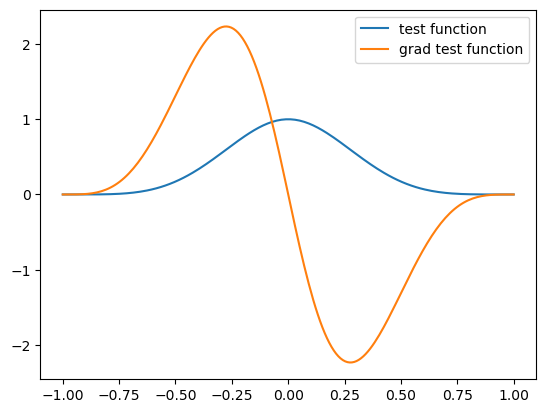
\includegraphics[width=0.6\linewidth]{./pics/final/possion/dgnet1d/WendlandCSRBFs.png}  
    \caption{Wendland's CSRBFs}
\end{figure} 
可以发现函数以及导数图像在边界处为0。

\subsubsection{约束组成(损失函数)}

参考单元的坐标记为$\boldsymbol{s}$,那么真实的物理区域有坐标仿射变换$\boldsymbol{x}=\boldsymbol{s} R_{i}+\boldsymbol{x}_{i}^{c}$, 将其代入上式残差形式中有:

$$\begin{aligned}
\mathcal{R}\left(u_{N N} ; \varphi_{i}\right) & =\int_{B\left(\boldsymbol{x}_{i}^{c}, R_{i}\right)} \nabla_{\boldsymbol{x}} u_{N N} \cdot \nabla_{r} \varphi_{i} \cdot \nabla_{\boldsymbol{x}} r d \boldsymbol{x}-\int_{B\left(\boldsymbol{x}^{c}, R_{i}\right)} f \varphi_{i} d \boldsymbol{x}, \\
& =R_{i}^{d}\left(\int_{B(\mathbf{0}, 1)} \nabla_{\boldsymbol{x}} u_{N N}(\boldsymbol{x}) \cdot \nabla_{r} \varphi_{i} \cdot \nabla_{\boldsymbol{x}} r d \boldsymbol{s}-\int_{B(\mathbf{0}, 1)} f(\boldsymbol{x}) \varphi_{i} d \boldsymbol{s}\right),
\end{aligned}$$

其中由链式法则  $\nabla_{\boldsymbol{x}} \varphi_{i}=\nabla_{r} \varphi_{i} \cdot \nabla_{\boldsymbol{x}} r$ .
文中在$B(\mathbf{0}, 1)$中随机选取了Nint个积分点,对$N_{p}$个积分区域进行数值积分,也即对$N_p$个小圆上积分。
假设$\left\{\boldsymbol{s}_{k}\right\}_{k=1}^{m}$为 $K_{i n t}$个积分点,且 $\left\{w_{k}\right\}_{k=1}^{m}$为对应的积分权重。
那么将  $\boldsymbol{x}_{k}^{(i)}$记作$\boldsymbol{s}_{k} * R_{i}+\boldsymbol{x}_{i}^{c}$。

则代理模型在单个圆上的损失函数为$\mathcal{R}\left(u_{N N} ; \phi_{i}\right)$可以写作:

$$\mathcal{R}\left(u_{N N} ; \varphi_{i}\right) \approx \frac{R_{i}^{d} V_{B(\mathbf{0}, 1)}}{K_{\text {int }}} \sum_{k=1}^{K_{\text {int }}} w_{k}\left(\nabla_{\boldsymbol{x}} u_{N N}\left(\boldsymbol{x}_{k}^{(i)}\right) \cdot \nabla_{r} \varphi_{i}\left(\boldsymbol{x}_{k}^{(i)}\right) \cdot \nabla_{\boldsymbol{x}} r\left(\boldsymbol{x}_{k}^{(i)}\right)-f\left(\boldsymbol{x}_{k}^{(i)}\right) \varphi_{i}\left(\boldsymbol{x}_{k}^{(i)}\right)\right),$$

若共取了$N_p$个圆进行particle loss的计算,则有
$$\mathcal{L}_{\mathcal{R}} \approx \frac{\mathcal{V}_{B(\mathbf{0}, 1)}^{2}}{N_{p} K_{i n t}^{2}} \sum_{i=1}^{N_{p}} R_{i}^{2 d}\left(\sum_{k=1}^{K_{\text {int }}} w_{k}\left(\nabla_{\boldsymbol{x}} u_{N N}\left(\boldsymbol{x}_{k}^{(i)}\right) \cdot \nabla_{r} \varphi_{i}\left(\boldsymbol{x}_{k}^{(i)}\right) \cdot \nabla_{\boldsymbol{x}} r\left(\boldsymbol{x}_{k}^{(i)}\right)-f\left(\boldsymbol{x}_{k}^{(i)}\right) \varphi_{i}\left(\boldsymbol{x}_{k}^{(i)}\right)\right)\right)^{2}$$

同时在边界上有约束
$$B= \sum_{j=1}^{N_{bd}}\left(u_{NN}(x_j) - g(x_j)\right)^2$$

因此最后损失函数可以设置为
$$\mathcal{L} = \mathcal{L}_{\mathcal{R}}+\mathcal{B}$$


\section{Split Weak Net}
在这里,我们受到DG方法中基函数选取的启发。由于基函数是定义在离散域上分片多项式函数,且数值解作为基函数的线性叠加。由广义逼近定理可以知道:
具有至少一个隐藏层的神经网络,在理论上可以以任意精度逼近任何连续函数。具体来说,对于一个足够大的隐藏层,神经网络可以以任意精度逼近任何连续函数。

因此想到在分片区域上利用局部小网络来替代原本局部线性方程组求解的过程;也就是说原来由一个整体的神经网络作为代理模型变为由多个小网络组成的代理模型。这样的做的优势我认为主要有以下几点:
\begin{itemize}
    \item 参数量由原来的多层神经网络参数$\Theta$变为单层网络参数$N_{\theta}\times N_{element}$
    \item 对于不规则边界,多尺度问题可以很自由的进行区域离散,分解操作
    \item 对于有间断解的问题允许交界面上的不连续
    \item 可以进行区域分解利用并行加速计算效率
\end{itemize}
在这里主要提出两种方案。
\subsection{Split Particle WNN}
该方法还是利用Particle WNN 的框架和思路,但是在这里,我们并不采取随机策略选取$N_p$个积分单元,而是根据区域离散(三角)化的结果进行选取。例如将区域$\Omega$离散化为$N_{elt}$个单元,则在单元中心作为圆心,半径不超过单元内切圆半径的长度作积分单元。
同理可以在每个积分单元上通过放射变换定义测试函数,这样依旧避免了边界上的积分。

设置每个单元上的小网络选择方案有两种,一种是为仅含有少量例如10个神经元的单隐藏层,激活函数为gelu的神经网络,第二种是在输入之后进行一个特征变换,例如输入为$(x,y)$,那么第一层的特征变换首先变为$(x, y, x^2, y^2,xy)$。
这里的特征变换和DeepONet中的Trunk Net类似,因此对于不同的问题可以选取不同的特征变换操作,例如对于涉及周期函数可以变为$\cos(x), \sin(x), \cos(y), \sin(x),\dots$,其实在这里设置特征变换的主要作用是为了增加网络拟合的非线性性,同时可以添加一些关于方程的先验知识。

接下来的Loss设置和Particle WNN类似,其中
$$\mathcal{L}_{\mathcal{R}} \approx \frac{\mathcal{V}_{B(\mathbf{0}, 1)}^{2}}{N_{elt} K_{i n t}^{2}} \sum_{i=1}^{N_{elt}} R_{i}^{2 d}\left(\sum_{k=1}^{K_{\text {int }}} w_{k}\left(\nabla_{\boldsymbol{x}} u_{net_i}\left(\boldsymbol{x}_{k}^{(i)}\right) \cdot \nabla_{r} \varphi_{i}\left(\boldsymbol{x}_{k}^{(i)}\right) \cdot \nabla_{\boldsymbol{x}} r\left(\boldsymbol{x}_{k}^{(i)}\right)-f\left(\boldsymbol{x}_{k}^{(i)}\right) \varphi_{i}\left(\boldsymbol{x}_{k}^{(i)}\right)\right)\right)^{2}$$

边界约束项为
$$B (u)= \sum_{e\in\mathscr{E}^D}\int_e(u_{net} - g)^2$$


我们记区域一共被分解成了$Nelt$个单元,在每个单元上定义网络$net_i$
但是,为了约束最终解的光滑性,我们添加惩罚项
$$J_0 = \sum_{e\in\mathscr{E}^I}\int_{e}[u]^2; \qquad J_1 = \sum_{e\in\mathscr{E}^I}\int_{e}[\nabla u \cdot \textbf{n}]$$

因此损失函数可以写为
$$\mathcal{L} = \mathcal{L}_{\mathcal{R}} + B+J_0+J_1$$

数值结果可行性见后面一章。
\subsubsection*{注:}
其实可以发现这里的Loss函数其实有四项,这里其实加大了网络优化的难度。但我认为分解成小网络区域,其实是解决区域之间耦合的方式,因此完全可以在解平滑的区域用粗网格离散,用大网络代理;在局部需要加密的地方用小网络进行替代,因此有时候优化难度大和离散化的方式也有很大关系。

\subsection{Split Discontinuous Galerkin Net}
其实可以看到Split Particle WNN 沿用了Particle WNN测试函数的选取策略,在紧支集为圆的函数空间上选取,这是一个很好的选择,避免了边界上不必要的积分。

然而在PWNN的文章中也提到,这种测试函数的选取对于不同的问题来说可能差异非常大,并且很大程度上影响着最后数值结果的精度,也就是说在某种程度上并不能够通过测试函数的选取方式进行精度的控制。

对于一些拥有振荡解的问题来说,PWNN往往通过增加随机选点的个数以及积分点的个数的方式来增加精度,这进一步增加了计算的复杂度。

考虑到在变分问题中,有限元类方法是非常强有力的工具。而对于有限元类方法三角划分是区域离散必不可少的一步,因此主要提出三种改进方案:

第一种解决方案是是否可以寻找紧支集为三角形的函数空间,替代紧支集为圆形的函数空间,从而不必随机选点,而是根据三角划分对于更需要的细化的地方进行加密取点。但这样的函数空间并不容易寻找。

第二种方案抛弃测试函数为单个的想法,接受边界上积分的麻烦。受到DG方法的启发,我们可以在单元上设置简单的基函数,例如设测试函数为分片多项式函数,则边界上的积分变得不可避免,但这对于间断有限元来说,并不困难。

第三种方案其实可以采取弱对抗神经网络中的策略,将测试函数取在神经网络函数空间中。但是由于是在每个小单元上取代理模型,因此测试函数数量会变大,训练会变得非常困难。

因此采取第二种方案。首先为和经典DG方法一样,将测试函数设分片多项式函数,例如2阶多项式,则Possion方程的弱解形式变为
$$-\int_\Omega \Delta u v = \int_\Omega fv$$
离散化之后可以写作
$$ -\sum_{E\in \Omega}\int_E \Delta u v = \sum_{E\in \Omega}\int_E fv $$
通过分部积分,对于单个单元E来说有:
$$\int_E \nabla u\cdot \nabla v - \int_{\partial E}(\nabla u\cdot \textbf{n})v = \int_E fv$$

因此
$$\begin{aligned}
    \mathcal{L}_{dg} =& \sum_{i=1}^{Nloc}\sum_{j=1}^{Nelt}\left(\int_{E_j} \nabla u_j\cdot \nabla \phi_i - \int_{\partial {E_j}}(\nabla u_j\cdot \textbf{n})\phi_i - \int_{E_j} f\phi_i\right)^2\\
    =&\sum_{i=1}^{Nloc}\sum_{j=1}^{Nelt}\left(\sum_{k=0}^{NintE}\left(w_k \nabla u_j \cdot \nabla \phi_i - f\phi_i\right)-\sum_{k=0}^{Ninte}w'_k(\nabla u_j \cdot \textbf{n})\phi_i\right)^2
\end{aligned}   
$$
其中Nloc为测试函数个数,NintE为区域上积分点个数,Kinte为内切面上积分点个数。

同理有边界约束项:
$$B (u)= \sum_{e\in\mathscr{E}^D}\int_e(u_{net} - g)^2$$

惩罚项
$$J_0 = \sum_{e\in\mathscr{E}^I}\int_{e}[u]^2; \qquad J_1 = \sum_{e\in\mathscr{E}^I}\int_{e}[\nabla u \cdot \textbf{n}]$$

因此损失函数可以写为
$$\mathcal{L} = \mathcal{L}_{dg} + \mathcal{B}+J_0+J_1$$

和之前的间断有限元方法相比,避免了复杂的稀疏矩阵计算,相反通过直接学习局部函数形式来代替求解基函数的系数。理论上来说我们可以通过控制测试函数个数$Nloc$来限制数值解的精度。







